% ============================================
\section{Modele i regresje}
% ============================================


\begin{frame}[t]{Model ML}

    \textbf{Stworzyliśmy prosty empiryczny model matematyczny,
        modelujący wysycający charakter wzrostu płacy nominalnej wraz z doświadczeniem zawodowym
        (związanym z podwyżkami, awansami ipd.):}

    \pause

    \begin{equation}
    k(x) = 1 + \alpha (1 - e^{-\beta x})
    \end{equation}
    \pause
    \\[.5cm]
    \centering
    $x$ --- lata doświadczenia w zawodzie
    \pause
    $\textrm{pensja} \pause = \textrm{pensja juniora} \pause \cdot k(x)$
\end{frame}

\begin{frame}[plain]
    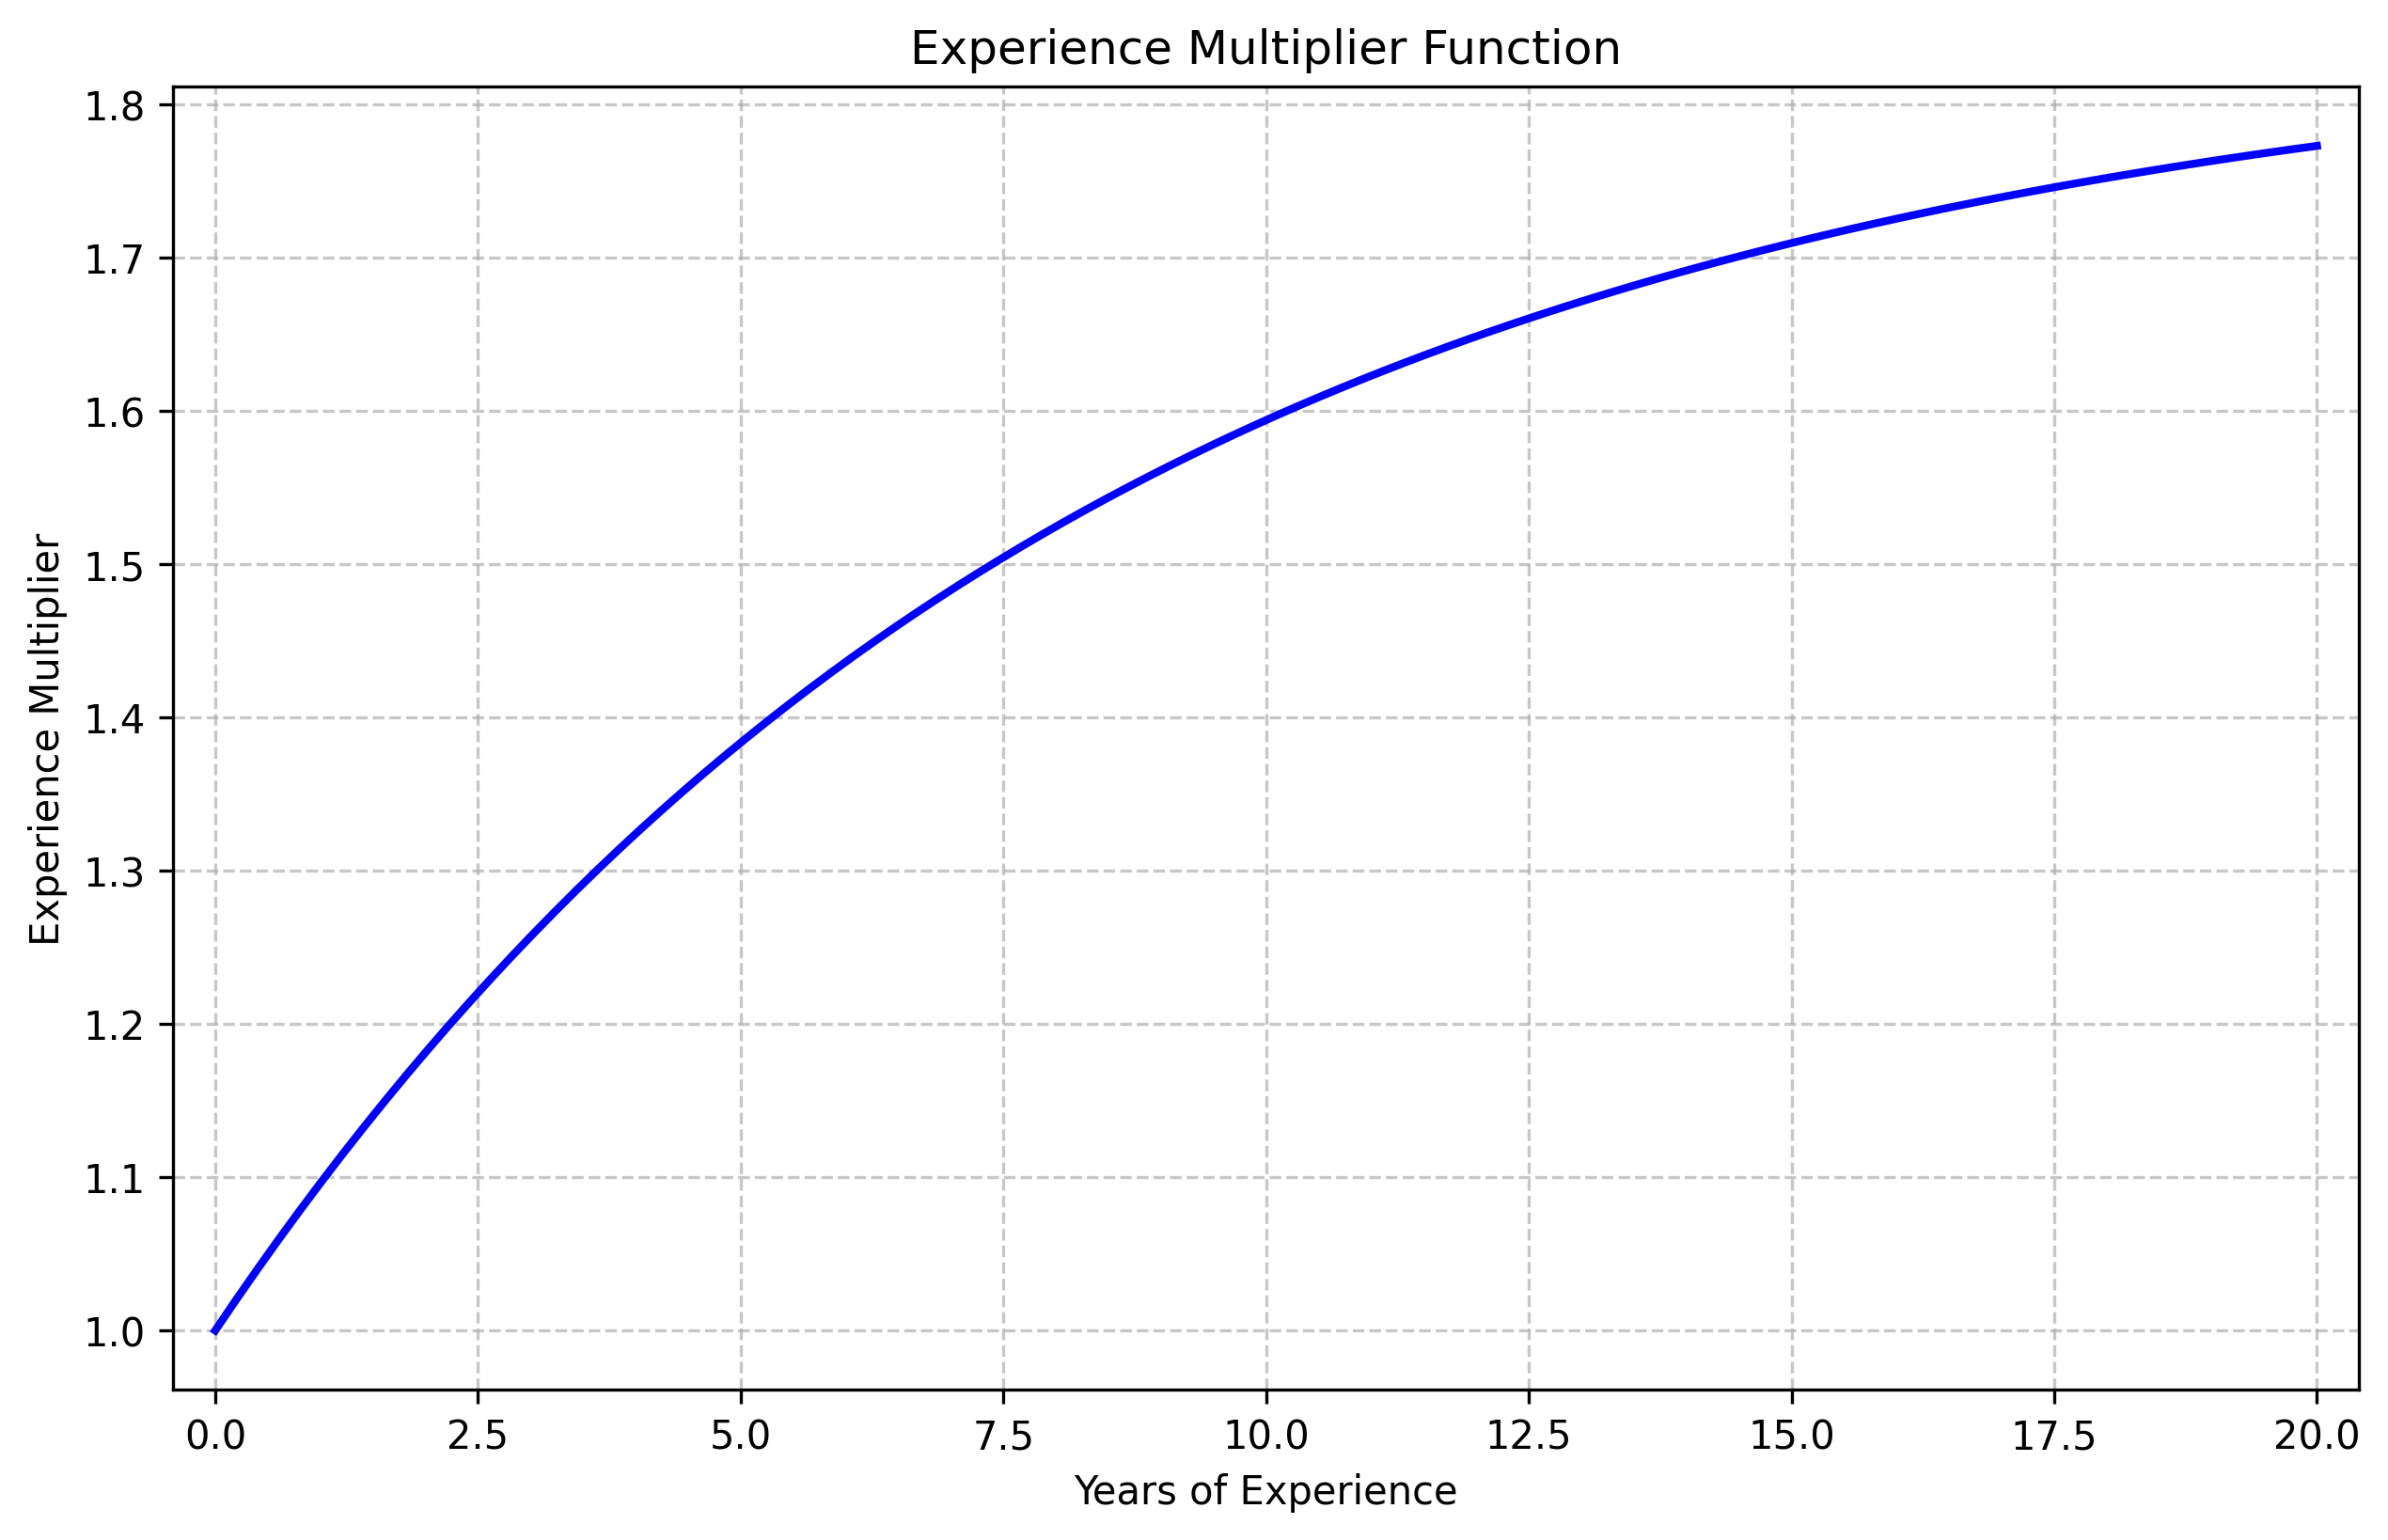
\includegraphics[width=.8\textwidth]{img/experience_multiplier}
\end{frame}

\begin{frame}[t]{Regresje dla rzeczywistych danych}
\centering
\begin{tabular}{cc}
    \pause
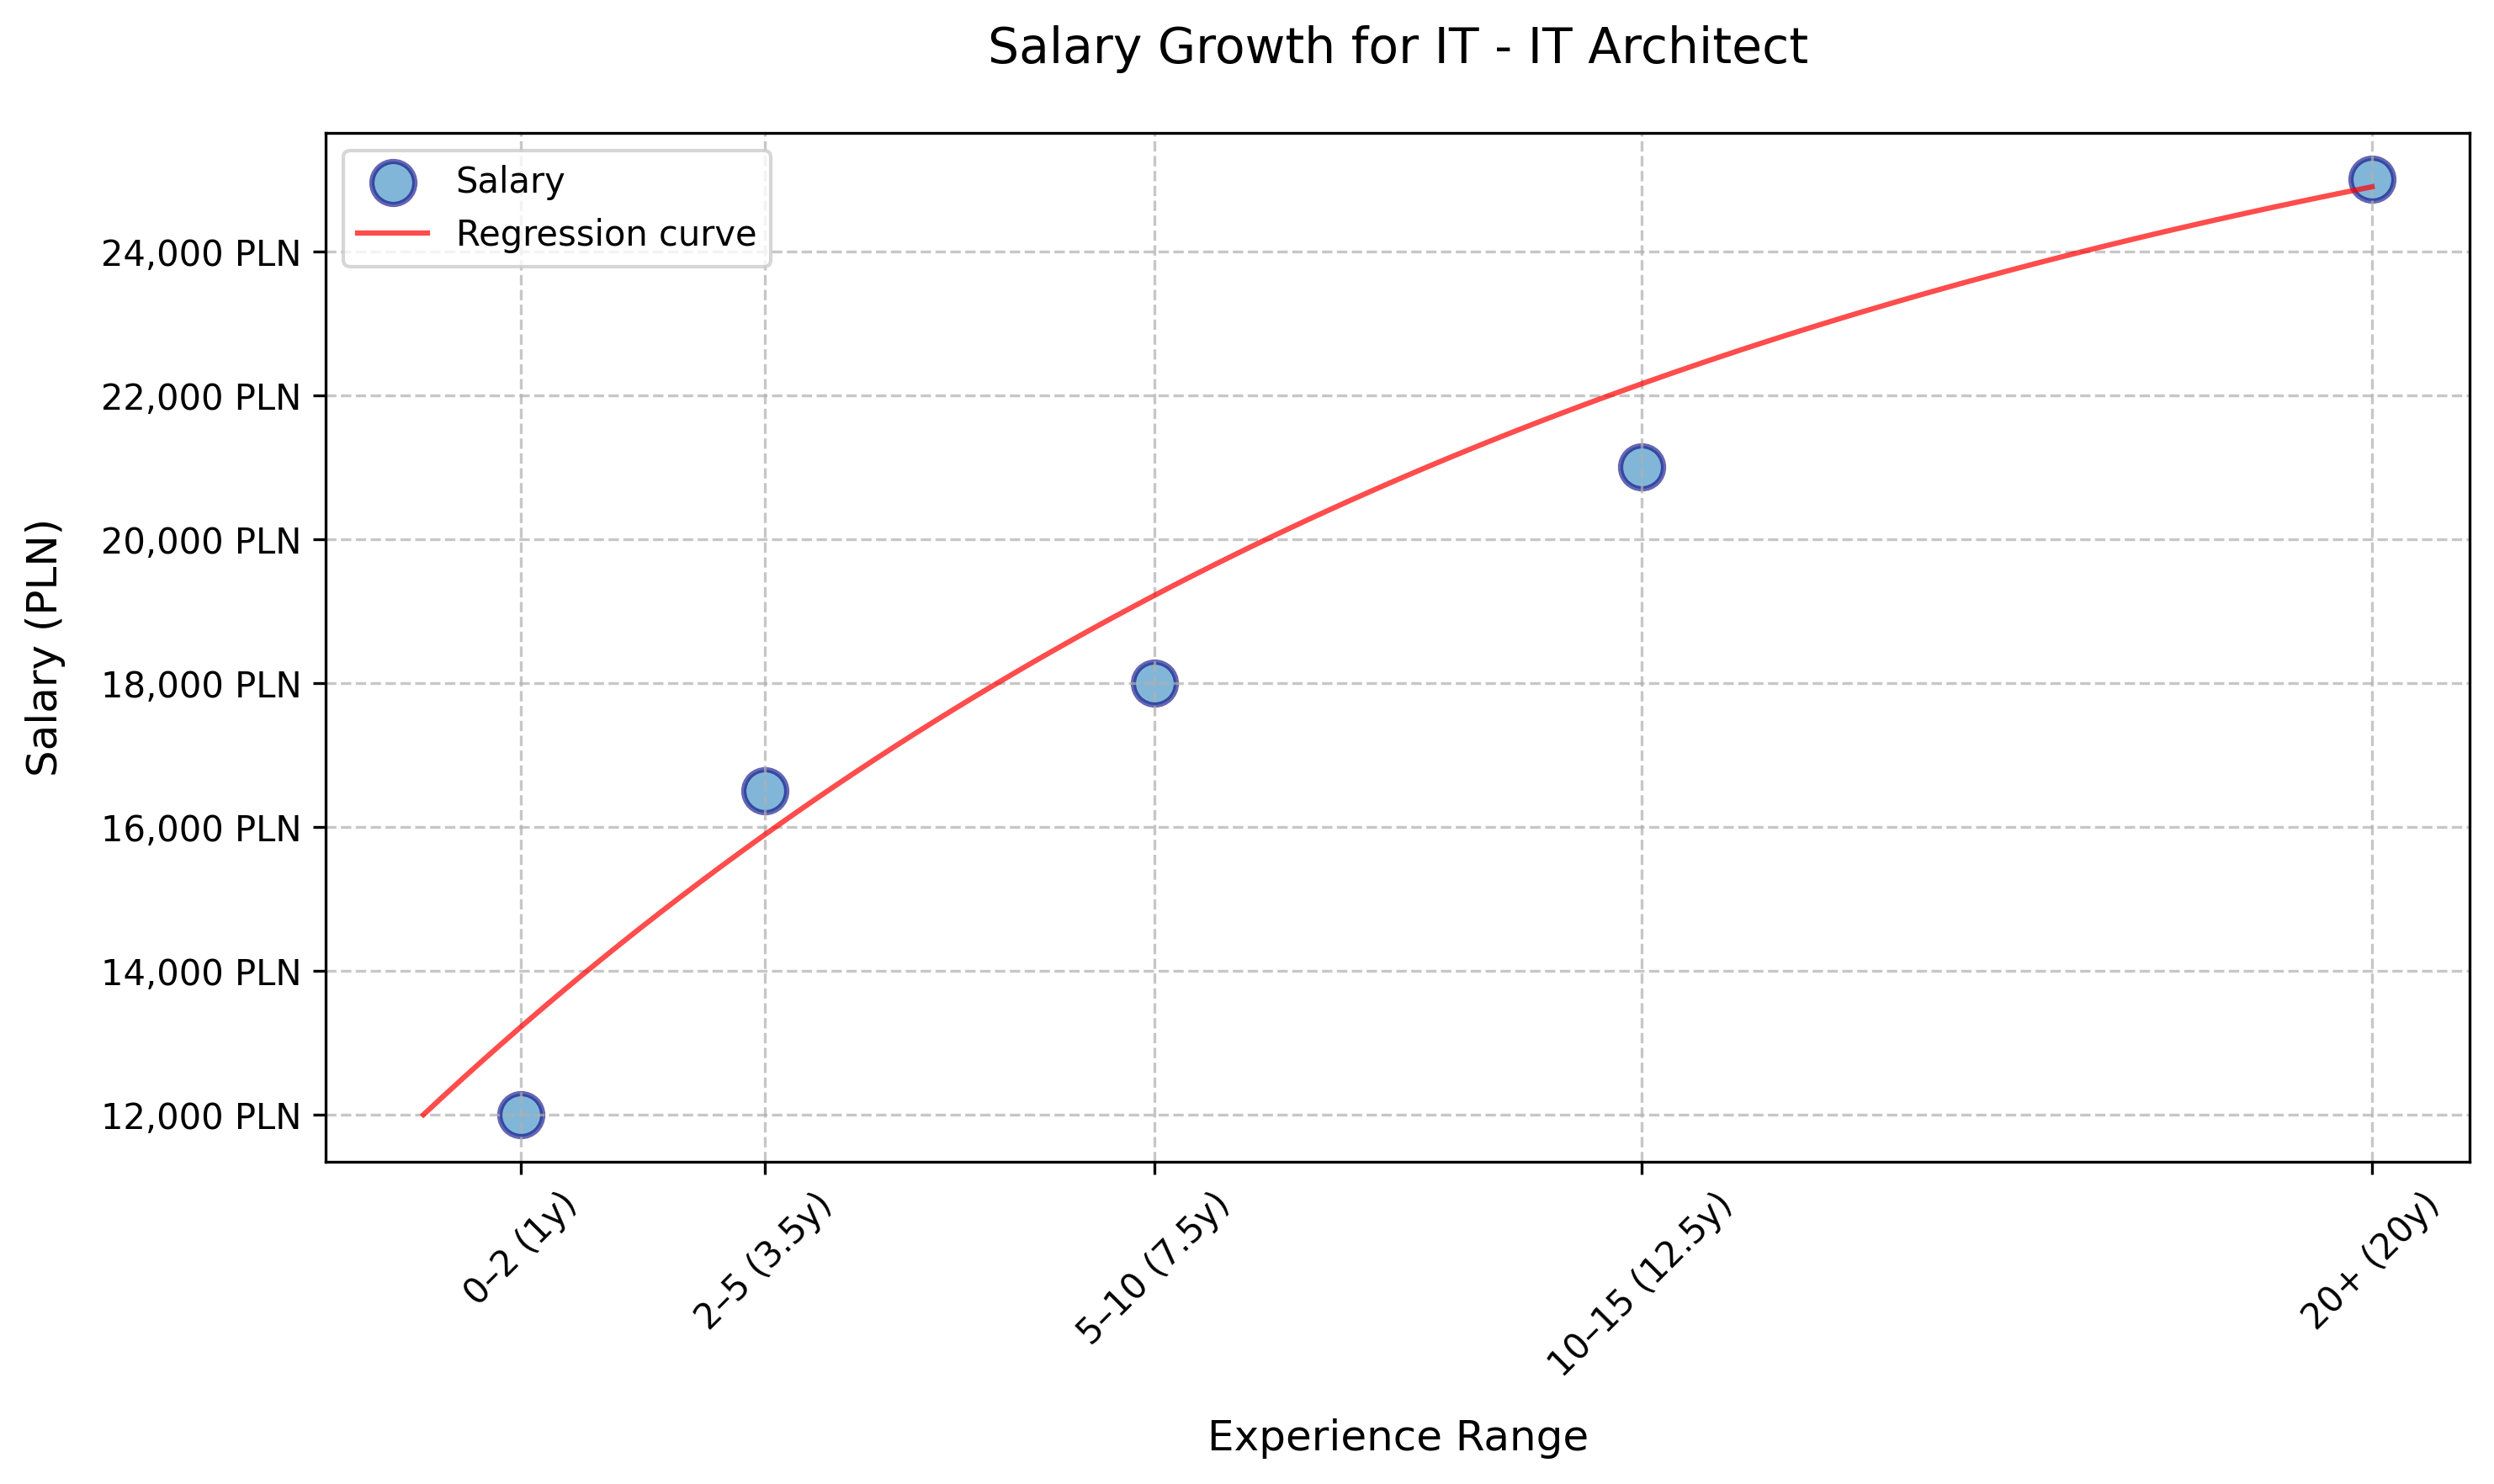
\includegraphics[width=0.45\linewidth]{img/salary_progression2} &
    \pause
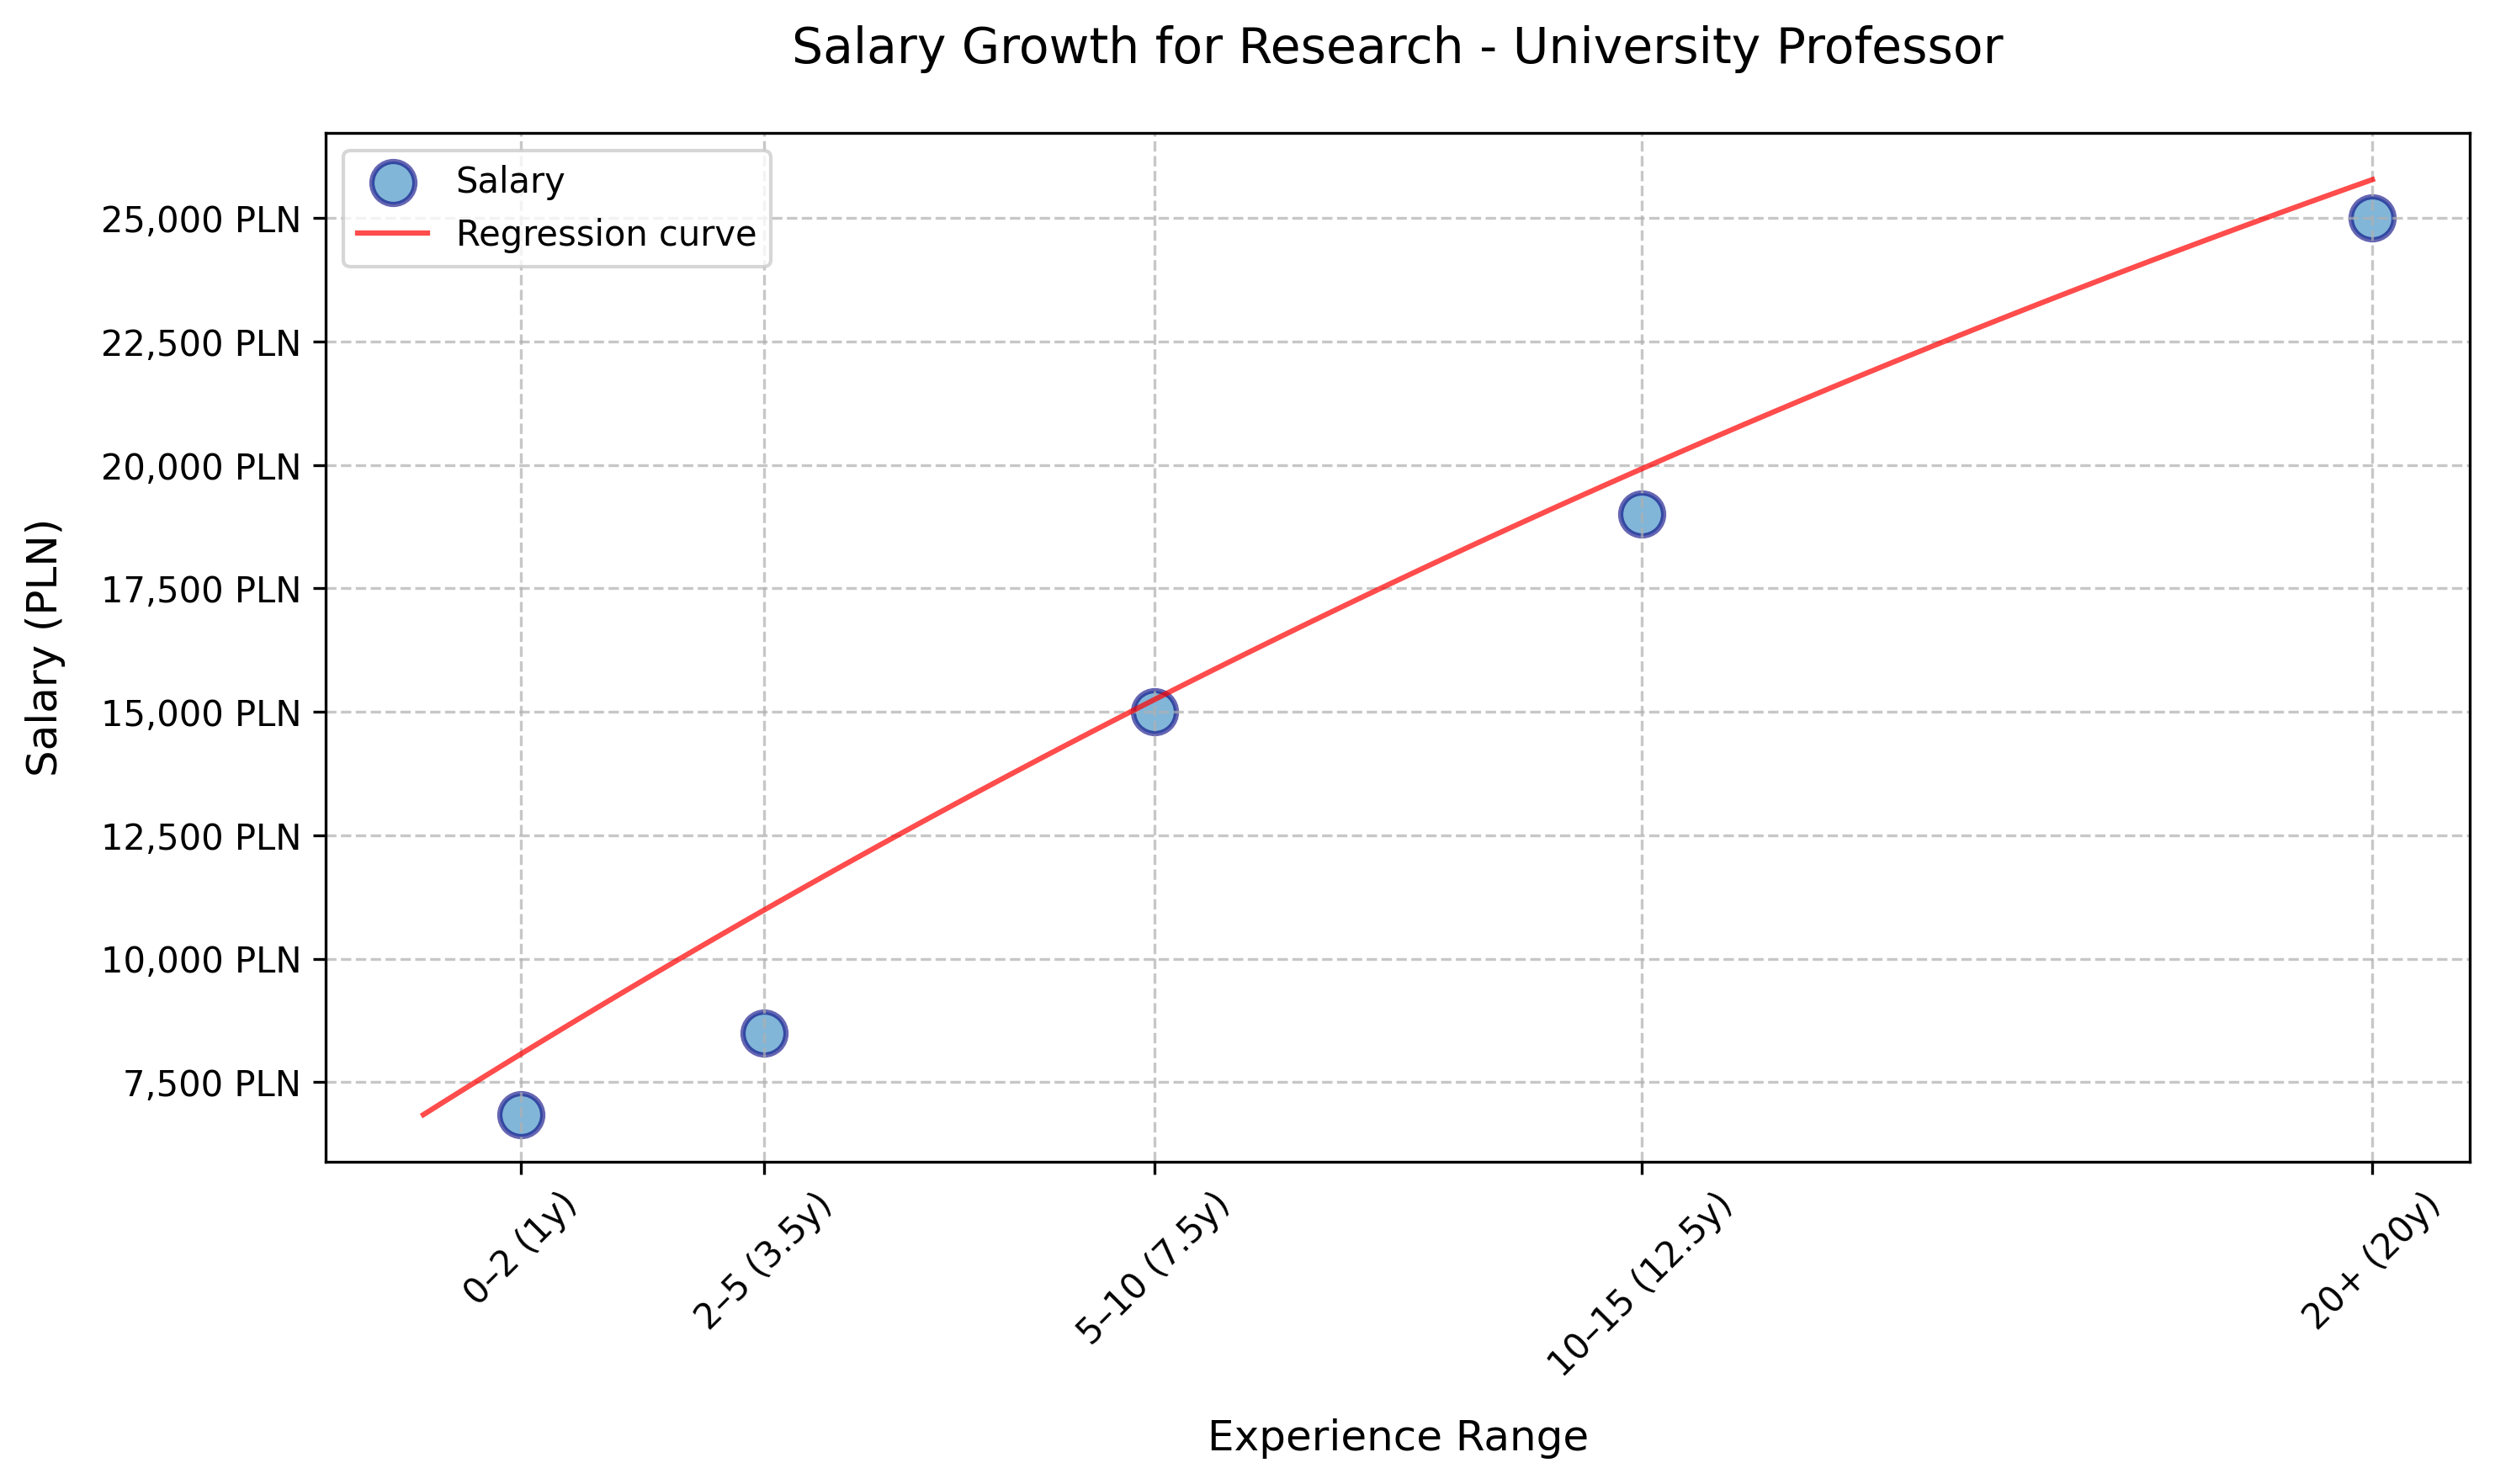
\includegraphics[width=0.45\linewidth]{img/salary_progression4} \\
    \pause
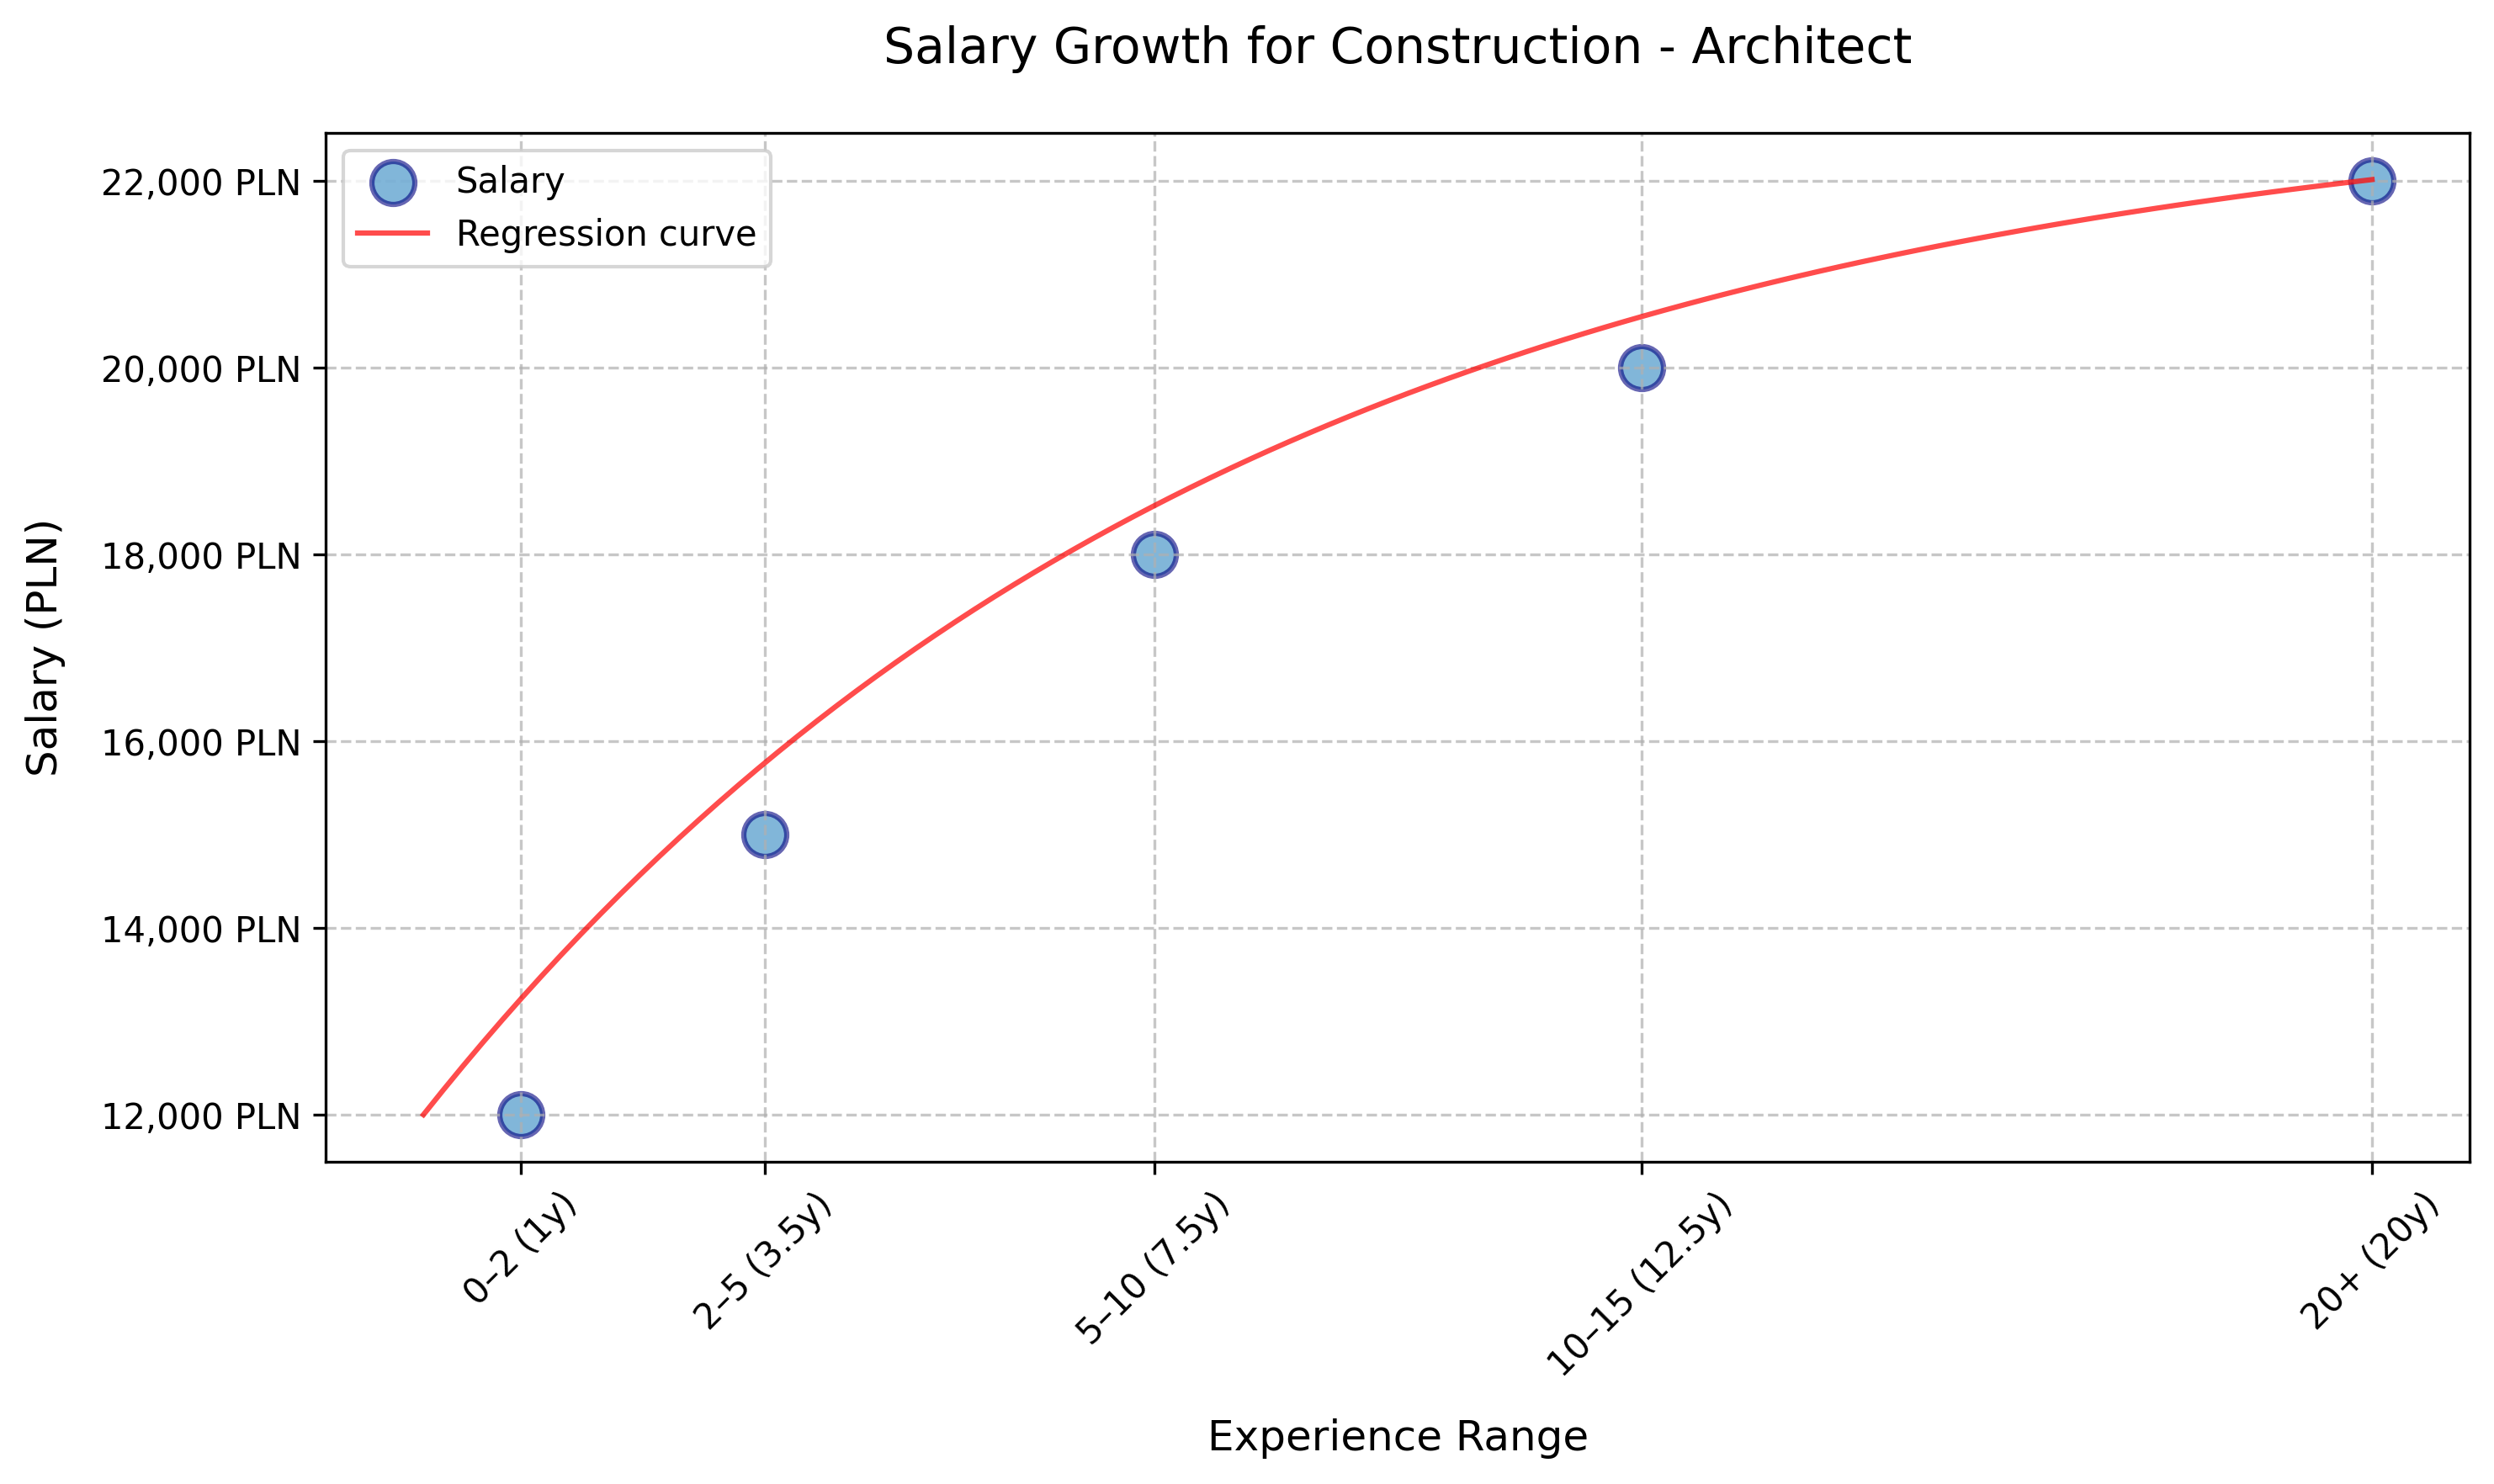
\includegraphics[width=0.45\linewidth]{img/salary_progression6} &
    \pause
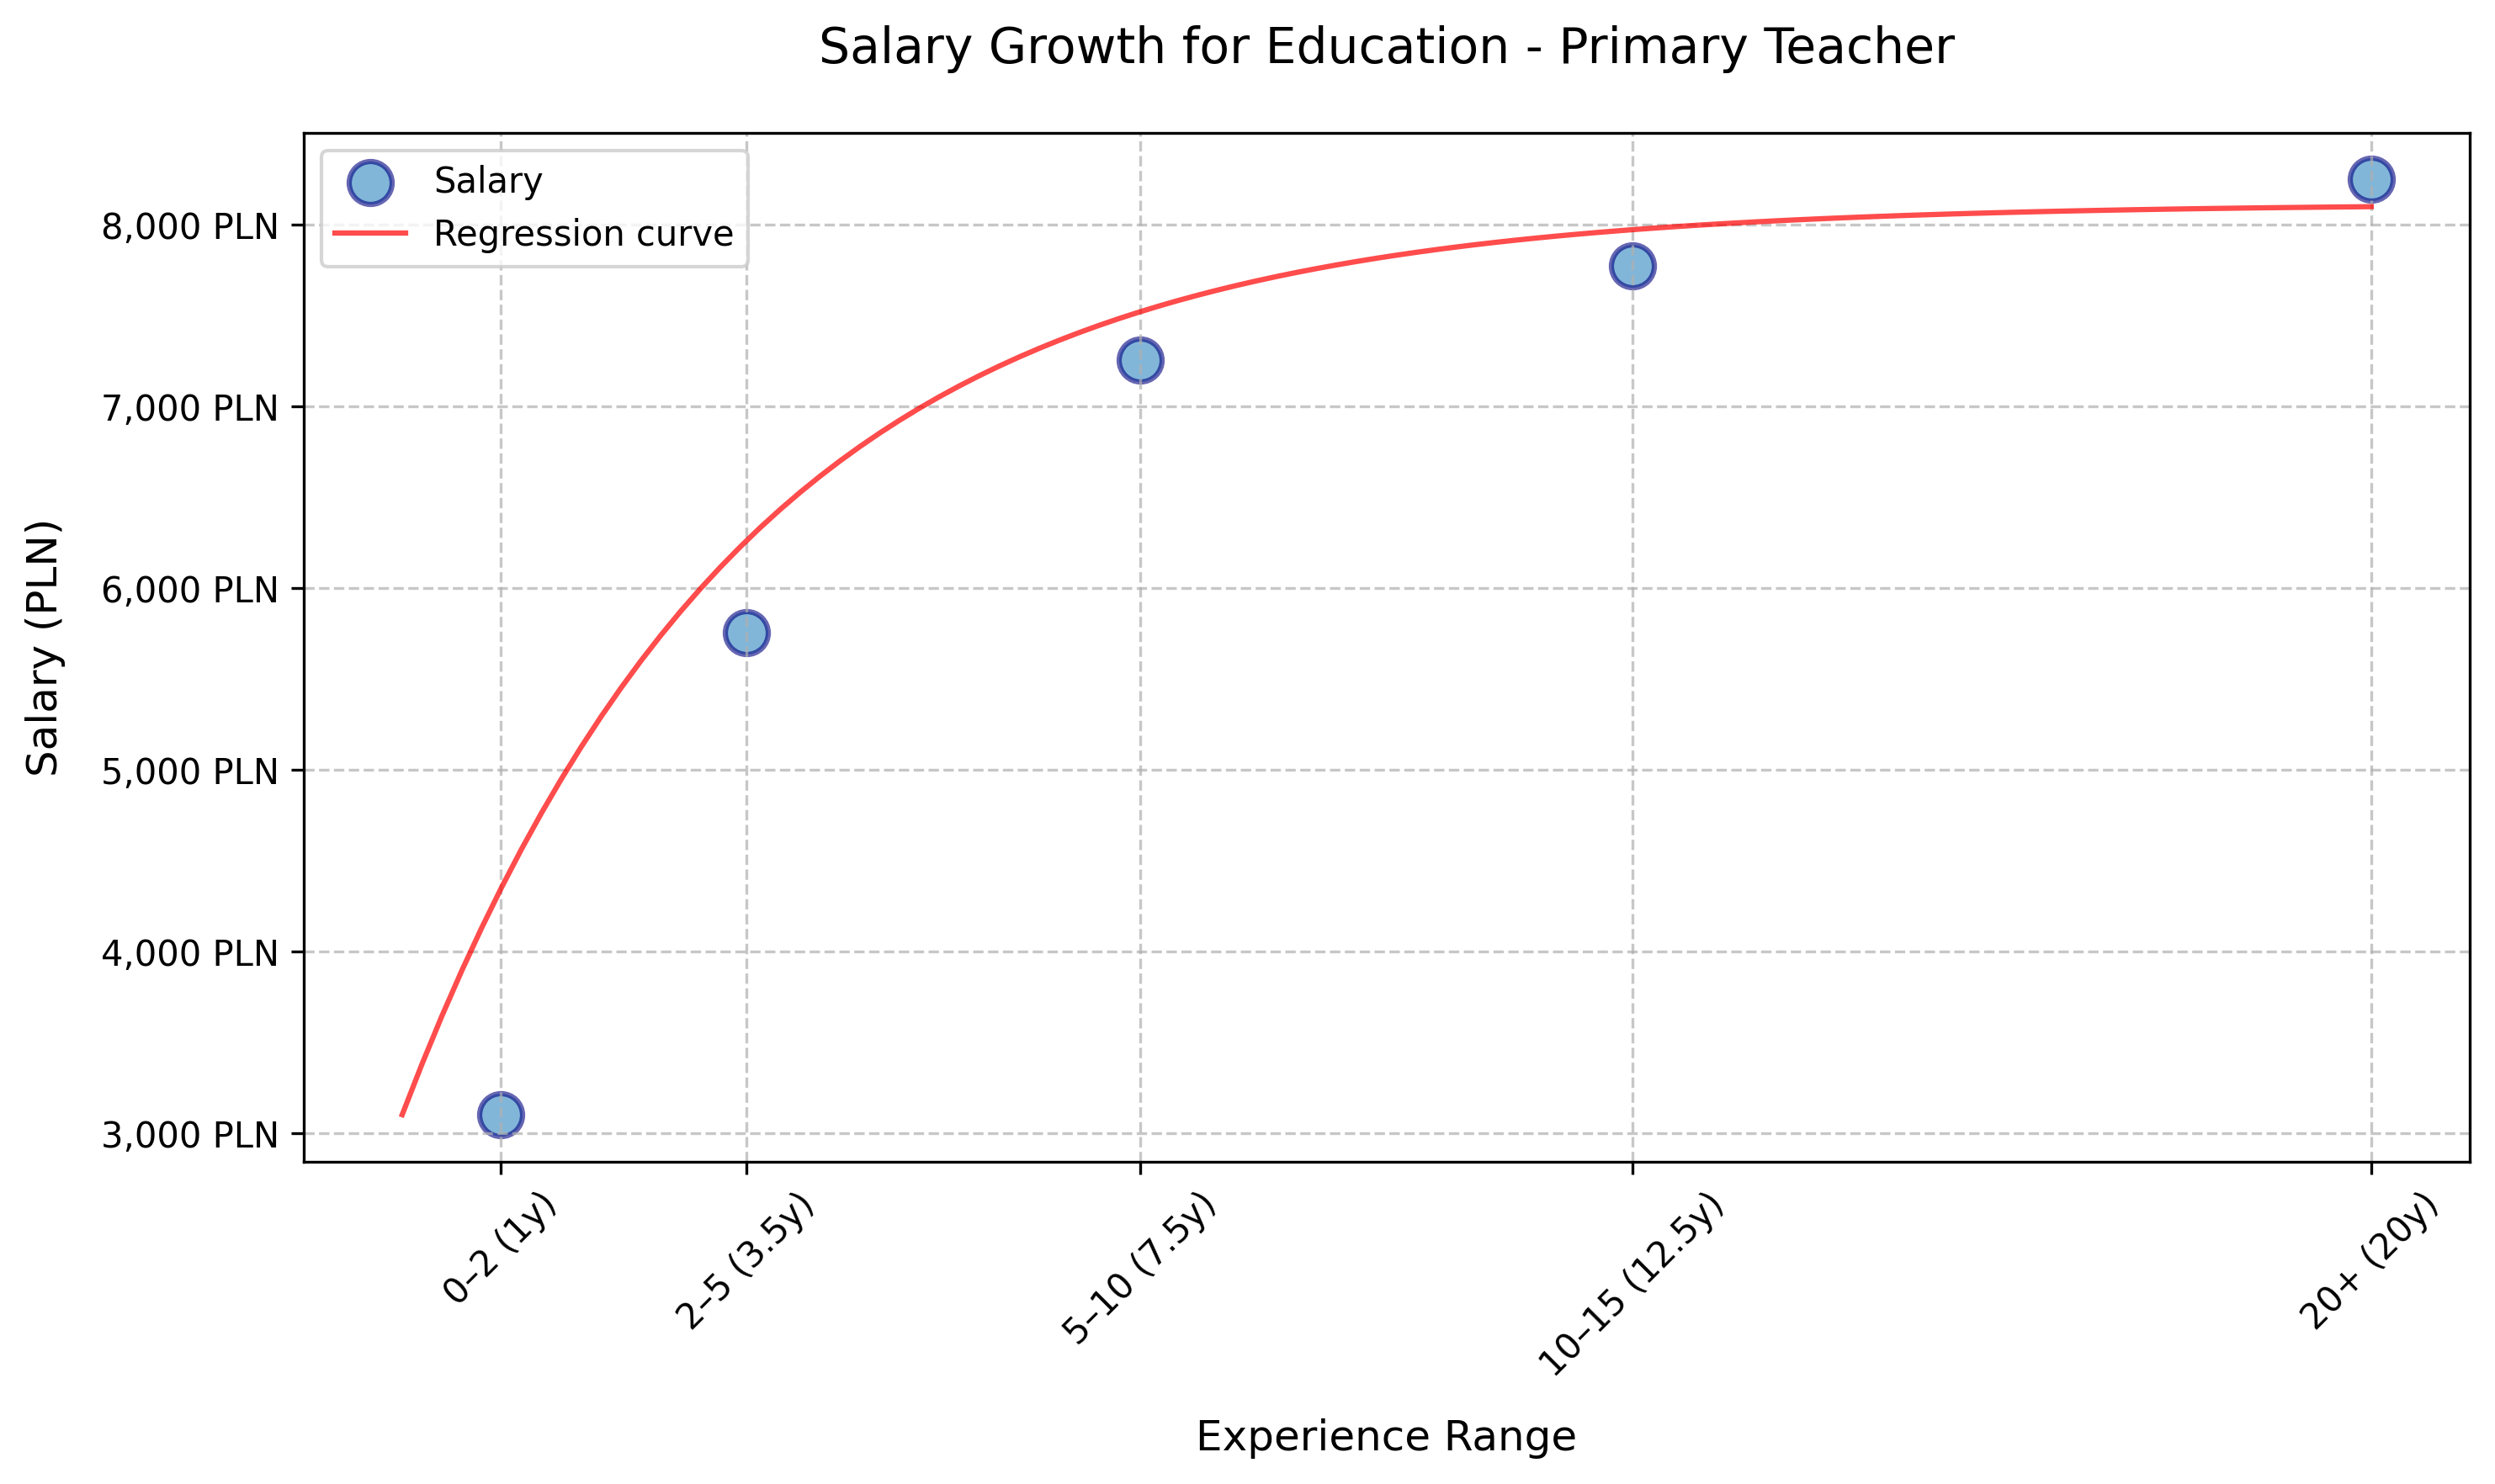
\includegraphics[width=0.45\linewidth]{img/salary_progression7}
\end{tabular}
\end{frame}

\begin{frame}[t]{LLM i RAG}{Klasyfikacja}
    \textbf{Wykorzystując API Gemini możemy dokonać klasyfikacji dowolnego zawodu do jednego,
        z uprzednio wytrenowanych modeli.}
    \\
    \pause
    \brand{Przy użyciu technologii RAG (\emph{Retrieval-Augmented Generation})
    znajdujemy aktualną stawkę osoby rozpoczynającej karierę (tzw. juniora) danej branży}
    \\
    \pause
    \highlight{Dokładając model czynników makroekonomicznych takich, jak inflacja czy przyrost PKB
    jesteśmy w stanie wiarygodnie oszacować całą finansową historię użytkownika - zarówno przeszłą jak i przyszłą!}
\end{frame}
